\section{Netztopologien}


\subsection{Strahlnetz}

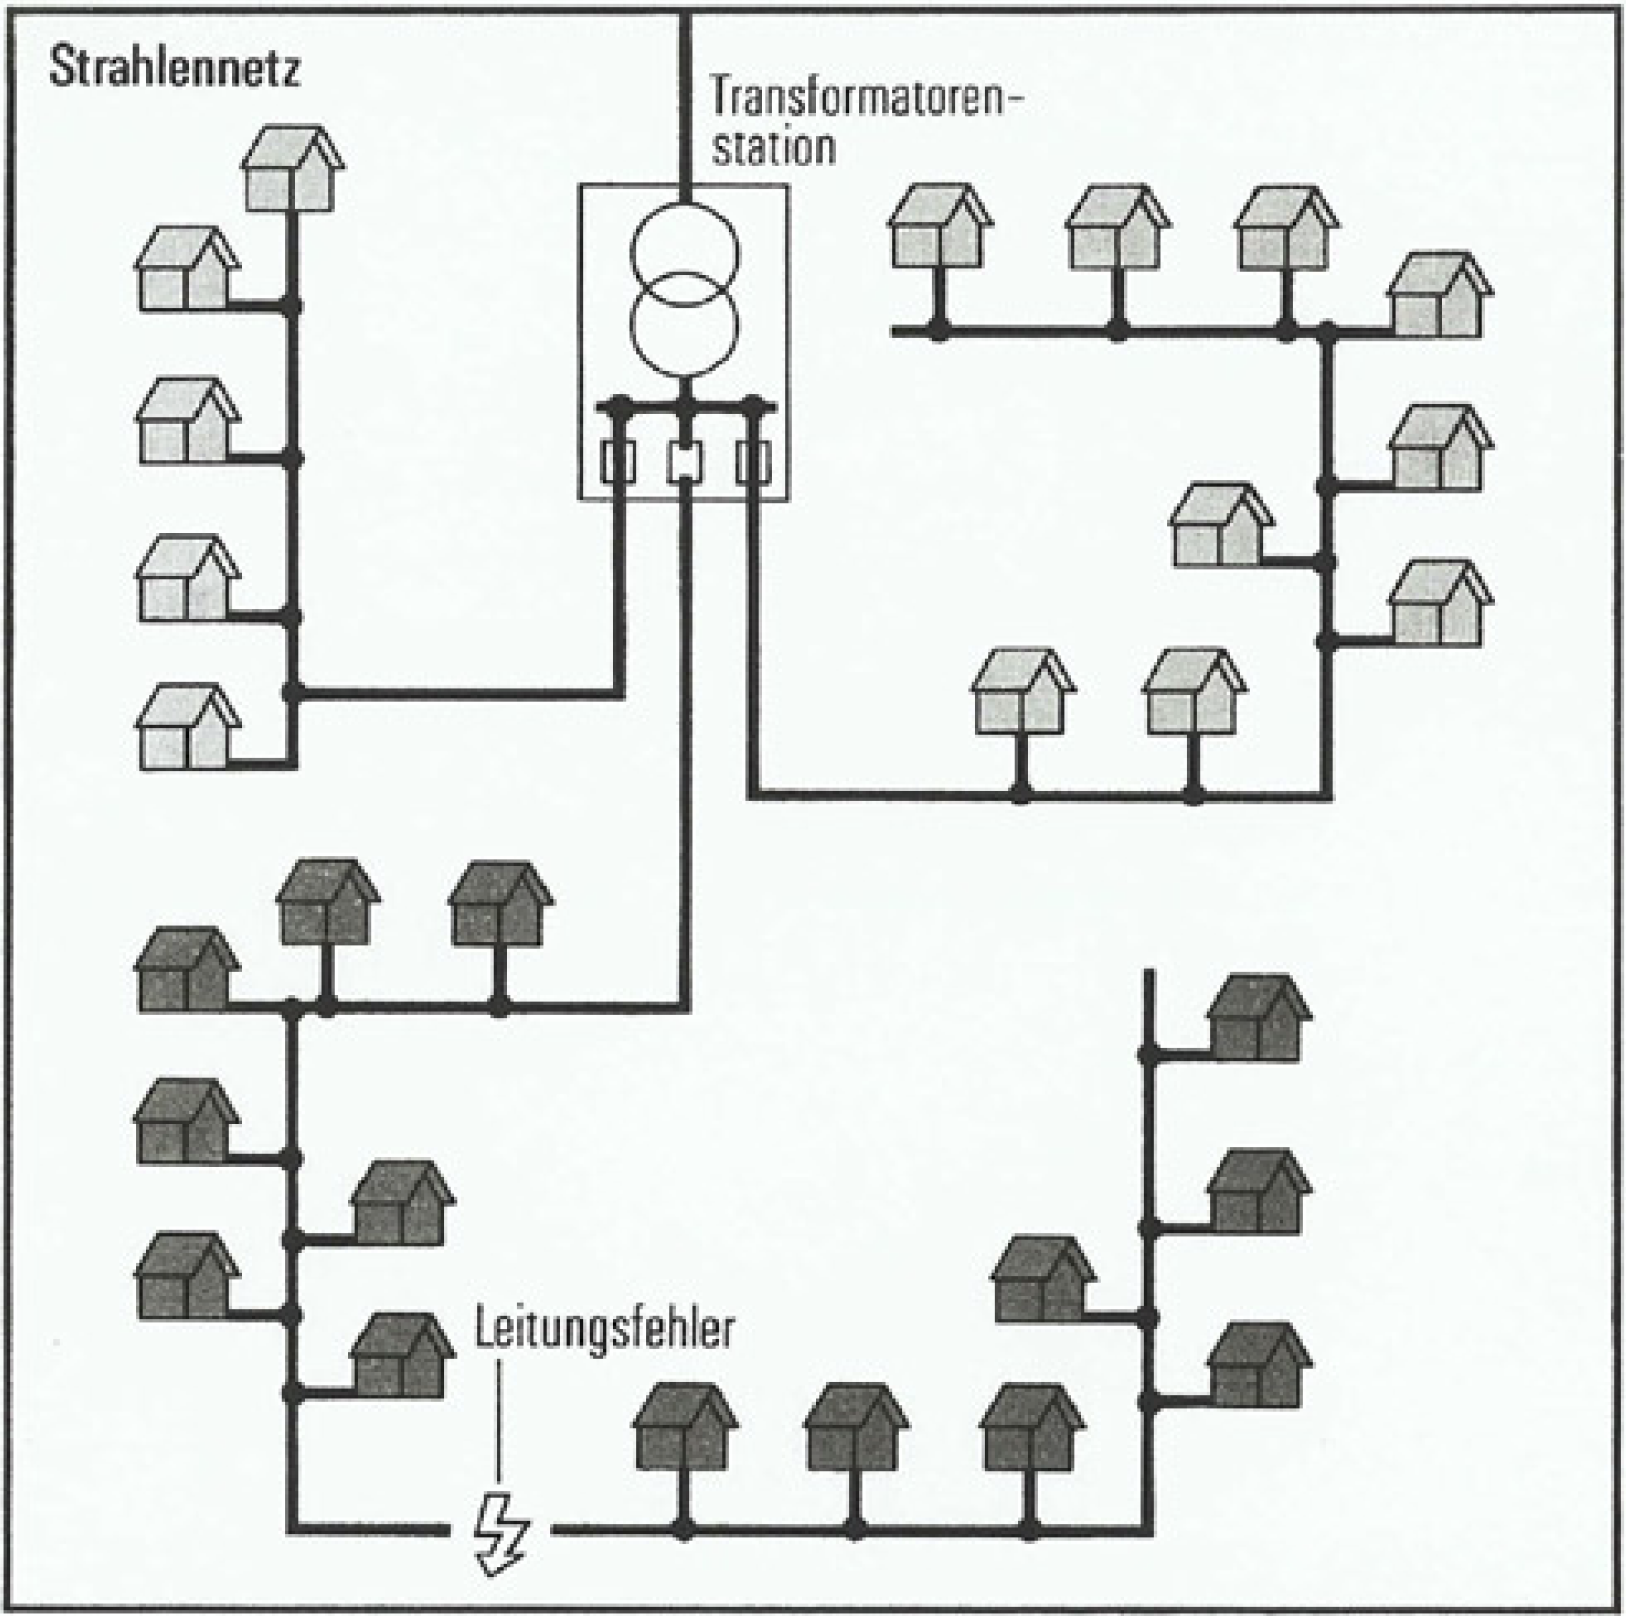
\includegraphics[width=0.55\columnwidth, align=c]{images/Strahlnetz.png}

\textbf{Pro:}
    \begin{itemize}
        \item geringer Planungsaufwand
        \item große Übersichtlichkeit bei der Fehlersuche
        \item geringe Anforderungen an den Netzschutz
    \end{itemize}
\vspace{1em}
\textbf{Contra:}
    \begin{itemize}
        \item größer werdende Spannungsabfälle mit zunehmendem Abstand von der Einspeisung
        \item höhere Leistungsverluste mit zunehmendem Abstand von der Einspeisung
    \end{itemize}


\subsection{Ringnetz}

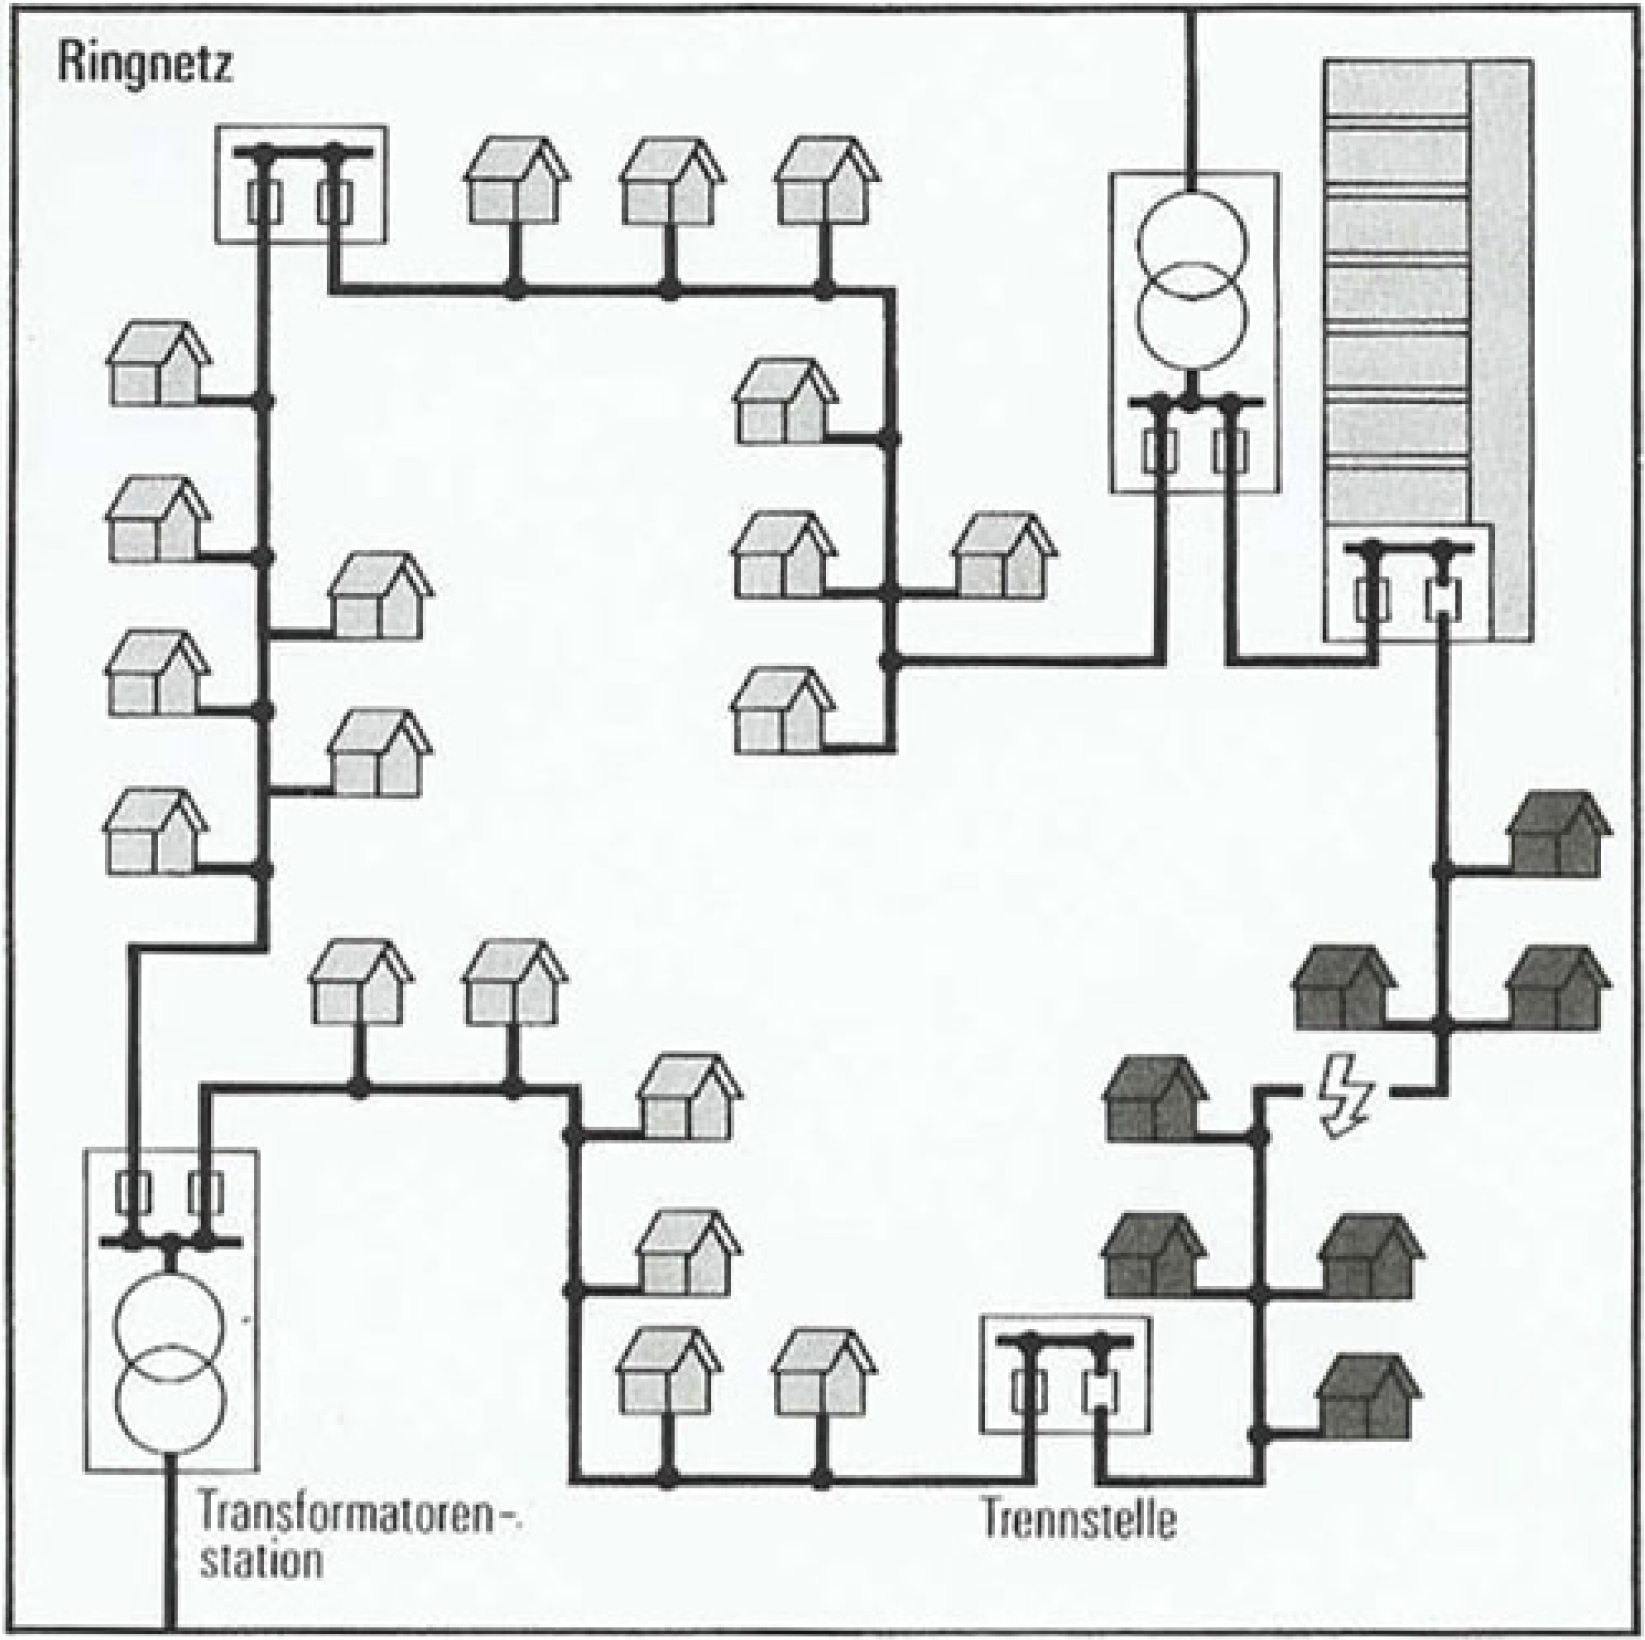
\includegraphics[width=0.55\columnwidth, align=c]{images/Ringnetz.png}

\textbf{Pro:}
\begin{itemize}
    \item höhere Versorgungssicherheit
    \item geringere Verluste
    \item verbesserte Spannungshaltung
\end{itemize}

\vspace{1em}
\textbf{Contra:}
\begin{itemize}
    \item höhere Anspruch an die Qualifikation des Wartungspersonals
\end{itemize}

\subsection{Maschennetz}

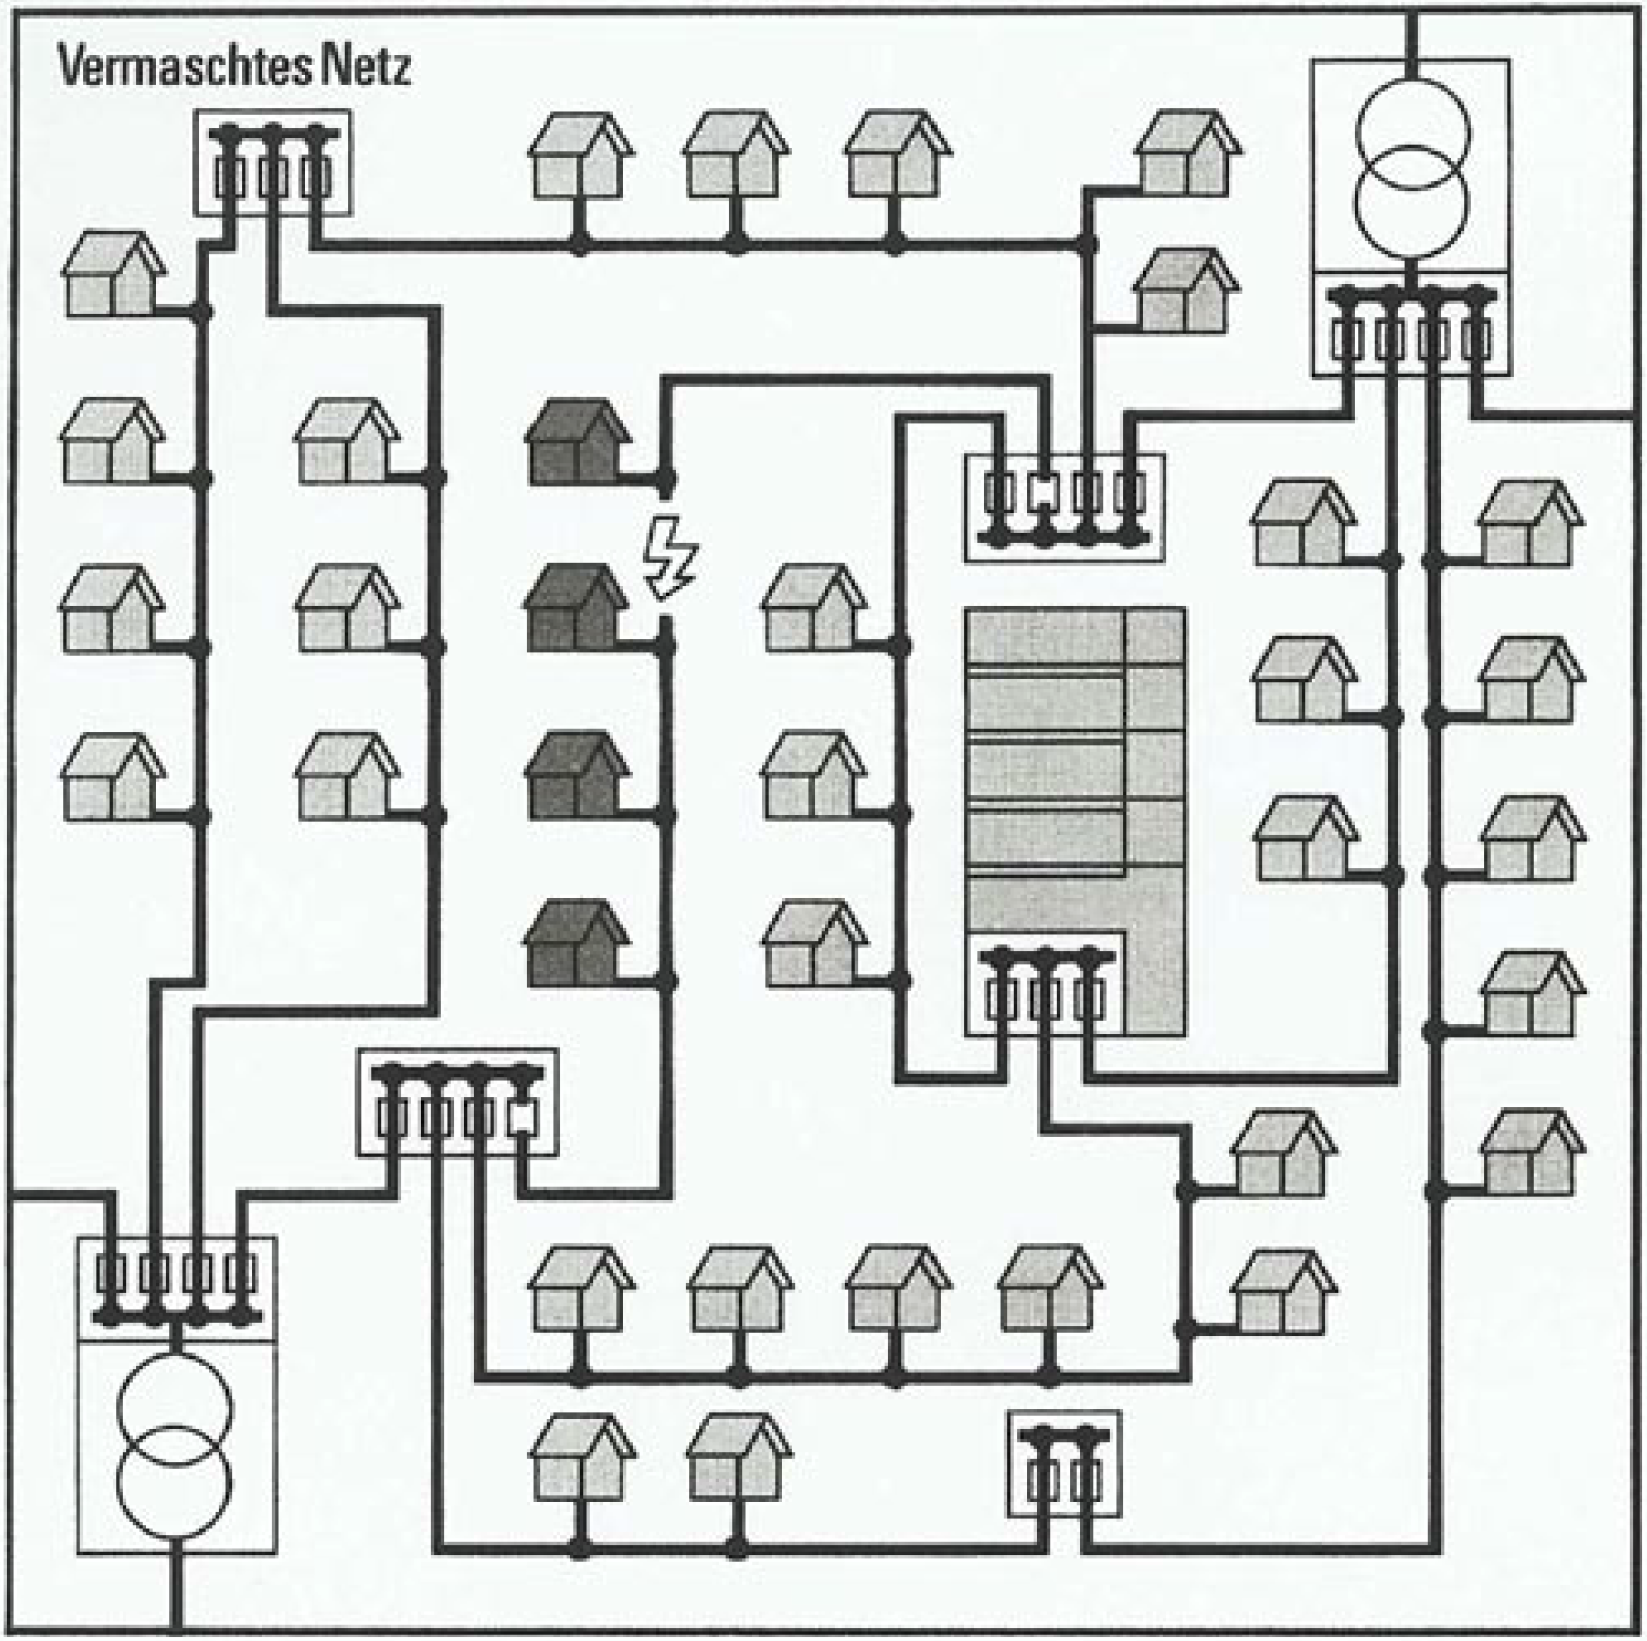
\includegraphics[width=0.55\columnwidth, align=c]{images/Maschennetz.png}

\textbf{Pro:}
\begin{itemize}
    \item eine optimale Versorgungszuverlässigkeit
    \item optimale Spannungshaltung
    \item minimale Leistungsverluste
\end{itemize}

\vspace{1em}
\textbf{Contra:}
\begin{itemize}
    \item hohe Investitionskosten
    \item hohe Projektions- und Wartungsaufwand
    \item höhere Kurzschlussströme
\end{itemize}













